\documentclass[11pt]{amsart}
\usepackage[a4paper,margin=1in]{geometry}
\usepackage{amsmath,amssymb,amsthm}
\usepackage{tikz}
\usetikzlibrary{decorations.pathreplacing}
\usepackage[hidelinks]{hyperref}

\newtheorem{thm}{Theorem}
\newtheorem{lemma}[thm]{Lemma}
\theoremstyle{definition}
\newtheorem{example}[thm]{Example}
\newtheorem{remark}[thm]{Remark}

\title[The moment of capture]{The moment of capture in a quadratic recurrence modulo 3}
\author{Vamshi Jandhyala}
\address{London, United Kingdom}
\subjclass[2020]{11B50, 11B37}
\keywords{recurrence modulo 3, eventual periodicity, pre-period, OEIS A112683}
\date{18 November 2026}

\begin{document}

\begin{abstract}
Fix $k\ge 2$ and let $x_1=\dots=x_{k-1}=0$, $x_k=1$ and $x_n=x_{n-1}+x_{n-k}^2$ in $\mathbb{Z}/3$. For many $k$
the sequence wanders for a very long time and then settles into a cycle of length $4$. Finch observed that the
settling always happens in the same way: if $z$ is the end of the first run of zeros spaced exactly four apart
that is long enough to force the cycle, and $\mu$ is the pre-period, then $z-\mu=6$. We prove this for every
$k\ge 3$ and show that it fails for $k=2$. The proof rests on one observation: inside the capturing run the rule
looks back exactly $k$ places, onto the stretch just before the run, so the run determines that stretch almost
completely, and minimality of $z$ does the rest. The theorem for $k\ge6$ and the counterexample at $k=2$ are
formalised in Lean; the case $k=3$ is checked by computation.
\end{abstract}

\maketitle

\section{Introduction}

Finch \cite{F26} studies three recurrences modulo $3$ built from squares of two earlier terms. For his rule (A),
fix $k\ge2$ and put
\[
x_1=\dots=x_{k-1}=0,\qquad x_k=1,\qquad x_n=x_{n-1}+x_{n-k}^2\quad(n\ge k+1),
\]
all in $\mathbb{Z}/3$. Since $c^2=1$ for $c\neq0$ and $0^2=0$, the rule says that at each step the sequence
either stays put or goes up by one, according as the term $k$ places back is zero or not:
\begin{equation}\label{eq:step}
x_n-x_{n-1}=b_{n-k},\qquad b_m=\begin{cases}1,& x_m\neq0,\\ 0,& x_m=0,\end{cases}\qquad(n\ge k+1).
\end{equation}
Every such sequence is eventually periodic. Its periods, computed by Harder \cite{F02} and listed in OEIS A112683
\cite{Sl}, begin $1,4,4,9,19,4,4,22,36,\dots$, and the value $4$ keeps returning. Pinch explained the fours
(quoted by Miller \cite{Mi}): when $k\equiv2\pmod4$ the cycle $0,1,1,2$ satisfies the rule, and when $k\equiv3\pmod4$ the cycle
$0,1,2,2$ does. Whether a given $k$ actually reaches its cycle is another matter: $k=18$ and $k=23$ do not.

When the cycle is reached, it can take a very long time. For $k=403$ the pre-period is about $10^{11}$
\cite{F26}. Finch gives an exact test for capture. Call a \emph{run with $g$ gaps starting at $r$} a stretch
with $r\ge k+1$, $x_r=x_{r+4}=\dots=x_{r+4g}=0$, and no other zero strictly between $r$ and $r+4g$. Put
$G=\lceil (k-1)/4\rceil$. Finch proves that the sequence follows the $4$-cycle from the end of any run with $G$
gaps \cite[Prop.~13]{F26}. The \emph{capture point} $z$ is the least end of such a run, and the
\emph{pre-period} $\mu$ is the least $\mu\ge0$ with $x_{n+4}=x_n$ for all $n>\mu$. Finch conjectured
\cite[Conj.~23]{F26} that $z-\mu=6$ whenever the period is $4$, having checked fifteen values of $k$ up to $403$:
the cycle is never reached earlier than the capturing run allows, and never with a stray mismatch after it. He
also reduced the claim to a condition on the terms just before the run \cite[Remark~24]{F26}.

\begin{thm}\label{thm:main}
Let $k\ge3$ with $k\equiv2$ or $3\pmod4$, and suppose that a capture point $z$ exists (equivalently, the
period is $4$). Then $\mu=z-6$. For $k=2$ the capture point is $z=9$ but $\mu=0$, so the statement fails.
\end{thm}

The case $k=2$ is degenerate: the sequence is $0,1,1,2,0,1,1,2,\dots$ from the start, while runs are only counted
from $r\ge k+1=3$. This counterexample is also recorded, with a Lean formalisation, in the public repository of
the Omega Institute \cite{Om}. For $k=3$ a direct computation gives $z=11$ and $\mu=5$. The content of the theorem is the case
$k\ge6$, proved in Section~\ref{sec:proof}. The residues $k\equiv2,3\pmod4$ are the ones for which a
$4$-cycle exists \cite[Prop.~12]{F26}.

\begin{example}\label{ex:six}
Take $k=6$, so $G=2$ and the cycle is $0,1,1,2$. The sequence is
\[
\underbrace{0\,0\,0\,0\,0\,1}_{x_1,\dots,x_6}\;1\,1\,1\,1\,1\,2\;0\,1\,2\;\mathbf{0}\,1\,2\,2\,\mathbf{0}\,1\,1\,2\,\mathbf{0}\;1\,1\,2\,0\cdots
\]
The first run with two gaps has zeros at $16,20,24$, so $z=24$. The block from $16$ to $20$ reads $0,1,2,2,0$ and
disagrees with the cycle in its middle entry; the block from $20$ to $24$ reads $0,1,1,2,0$ and agrees. The last
$n$ with $x_n\neq x_{n-4}$ is $n=22$, so $\mu=18=z-6$. Figure~\ref{fig:look} shows why the two middle entries
differ: $x_{22}$ looks back to $x_{16}=0$ inside the run, while $x_{18}$ looks back to $x_{12}=2$, before it.
\end{example}

\begin{figure}[ht]
\centering
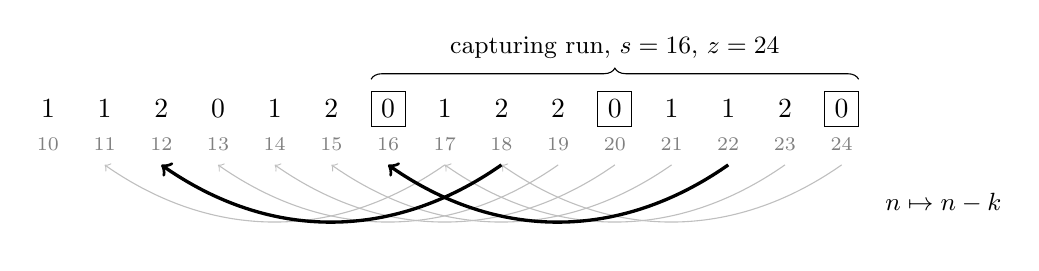
\begin{tikzpicture}[x=0.72cm,y=0.75cm]
  \foreach \n/\v in {10/1,11/1,12/2,13/0,14/1,15/2,16/0,17/1,18/2,19/2,20/0,21/1,22/1,23/2,24/0} {
    \node[font=\scriptsize,gray] at (\n,-0.6) {\n};
    \node at (\n,0) {$\v$};
  }
  \foreach \n in {16,20,24} { \draw (\n-0.3,-0.3) rectangle (\n+0.3,0.3); }
  \draw[decorate,decoration={brace,amplitude=4pt}] (15.7,0.5) -- (24.3,0.5)
    node[midway,above=4pt,font=\small] {capturing run, $s=16$, $z=24$};
  \foreach \n in {17,19,20,21,23,24} { \draw[->,gray!50,bend left=35] (\n,-0.95) to (\n-6,-0.95); }
  \foreach \n in {18,22} { \draw[->,very thick,bend left=35] (\n,-0.95) to (\n-6,-0.95); }
  \node[font=\small,anchor=west] at (24.6,-1.6) {$n\mapsto n-k$};
\end{tikzpicture}
\caption{The case $k=6$. Each step inside the run looks back six places (arrows below the positions; the two that matter are bold). The
run's own shape therefore fixes whether $x_{11},\dots,x_{18}$ are zero; minimality of $z$ then forces
$x_{12}\neq0$, which makes $x_{18}$ differ from $x_{22}$.}
\label{fig:look}
\end{figure}

\section{Proof of Theorem~\ref{thm:main} for $k\ge6$}\label{sec:proof}

The route is short. Inside the capturing run every step looks back exactly $k$ places, and since the run is
long, those look-backs land on the stretch just before it; so the shape of the run dictates which earlier
terms are zero (Steps~1 and~3). If the run could be pushed back by one block it would end earlier, so
minimality of $z$ fixes the one term the run leaves free (Step~4). That term decides the middle entry of the
block before the last, which therefore disagrees with the cycle (Step~5), while the last block and everything
after it agree (Steps~2 and~6). Example~\ref{ex:six} and Figure~\ref{fig:look} show all of this at $k=6$.

Write $k=4t+2$ or $k=4t+3$ with $t\ge1$. In both cases $G=t+1$. Let $s=z-4G$ be the first zero of the capturing
run, so $z=s+4t+4$, and
\begin{equation}\label{eq:zk}
z-k=s+2\quad(k=4t+2),\qquad z-k=s+1\quad(k=4t+3).
\end{equation}
Inside a run every block from one zero to the next reads $0,1,*,2$ with $*\in\{1,2\}$ \cite[Lemma~17]{F26}:
by \eqref{eq:step} each of its four steps is $0$ or $1$, the first step leaves $0$ for a nonzero value, so it is
$1$, and the last arrives at $0$ from a nonzero value, so it leaves $2$. Reading the four steps of the block
starting at $m\in\{s,s+4,\dots,z-4\}$ through \eqref{eq:step} gives
\begin{equation}\label{eq:block}
b_{m+1-k}=1,\qquad b_{m+4-k}=1,\qquad b_{m+2-k}+b_{m+3-k}=1,\qquad x_{m+2}=1+b_{m+2-k}.
\end{equation}
The first two say that the steps into and out of the zeros are forced; the third, that exactly one of the two
middle steps is a rise; the last, that the middle entry is $1$ exactly when the term $k$ places back is zero.

\emph{Step 1: the run starts late.} Taking $m=s$ in \eqref{eq:block} gives $b_{s+1-k}=1$. Since $b_n=0$ for
$n\le k-1$, we get $s+1-k\ge k$, that is, $s\ge2k-1$. In particular $s-4\ge k+1$.

\emph{Step 2: the last block agrees with the cycle.} By \eqref{eq:step} and \eqref{eq:zk}, for $k=4t+2$ the step
into $x_{z-2}$ is $b_{z-2-k}=b_s=0$, so $x_{z-2}=x_{z-3}=1$; for $k=4t+3$ the step into $x_{z-1}$ is
$b_{z-1-k}=b_s=0$, so $x_{z-2}=x_{z-1}=2$. In both cases $x_{z-2}$ equals the value of the cycle at that phase.

\emph{Step 3: the stretch before the run.} This is the look-back of Figure~\ref{fig:look}. Apply
\eqref{eq:block} to the last two blocks, $m=z-4$ and $m=z-8$
(the latter exists because $G\ge2$). With \eqref{eq:zk} this gives, for $k=4t+2$,
\[
b_{s-1}=b_{s-2}=1,\qquad b_{s-4}+b_{s-3}=1,
\]
and for $k=4t+3$, using $b_s=0$ in the pair $b_{s-1}+b_s=1$,
\[
b_{s-1}=b_{s-2}=b_{s-3}=1,\qquad b_{s-5}+b_{s-4}=1.
\]

\emph{Step 4: the run cannot be extended backwards.} Suppose $x_{s-4}=0$. In both cases Step~3 then makes
$x_{s-3},x_{s-2},x_{s-1}$ nonzero (for $k=4t+2$ through the pair $b_{s-4}+b_{s-3}=1$). So $s-4,s,s+4,\dots,z-4$ is
a run with $G$ gaps, and it starts at $s-4\ge k+1$ by Step~1. It ends at $z-4$, contradicting the minimality of
$z$. Hence $x_{s-4}\neq0$.

\emph{Step 5: the block before the last disagrees.} The middle entry of the block at $m=z-8$ is
$x_{z-6}=1+b_{z-6-k}$. For $k=4t+2$, $z-6-k=s-4$ and $b_{s-4}=1$, so $x_{z-6}=2\neq1=x_{z-2}$. For $k=4t+3$,
$z-6-k=s-5$, and $b_{s-5}=0$ by Step~3 and Step~4, so $x_{z-6}=1\neq2=x_{z-2}$.

\emph{Step 6: nothing disagrees afterwards.} We show $x_{n+4}=x_n$ for every $n\ge z-5$, by induction on $n$.
For $n=z-5$ both terms are the last entries $2$ of the final two blocks, and for $n=z-4$ both are zeros of the
run. For $n\ge z-3$, \eqref{eq:step} and the induction hypothesis $x_{n+3}=x_{n-1}$ reduce the claim to
$b_{n+4-k}=b_{n-k}$. If $n-k\ge z-5$ this is the induction hypothesis again. Otherwise $p=n-k$ lies between
$z-3-k$ and $z-6$, that is, between $s-1$ (resp.\ $s-2$) and $z-6$ by \eqref{eq:zk}. If $p\ge s$, both $p$ and
$p+4$ lie in the run, where $x_m=0$ exactly when $m\equiv s\pmod 4$. If $p<s$, then $b_p=1$ by Step~3, and
$p+4\in\{s+2,s+3\}$ is a nonzero position of the run.

By Steps~5 and~6 the last $n$ with $x_n\neq x_{n-4}$ is $n=z-2$, so $\mu=z-6$. \qed

Step~4 recovers Finch's Remark~24: for $k\equiv2\pmod4$ the capturing run is preceded by $x_{s-4}\neq0$, and for
$k\equiv3\pmod 4$ by $x_{s-5}=0$ and $x_{s-1}\neq0$. The proof never uses Finch's capture criterion: Step~6
reproves the part of it that is needed. Nor does it use the period: the identity holds whenever a run with $G$
gaps exists, which is what makes the period $4$.

\begin{remark}
Step~1 is far from sharp in practice. For the twenty-one capturing values $6\le k\le60$, $s-k$ is at least
$10$, and usually much larger: for $k=58$, $s=17760$.
\end{remark}

\section{Verification}

For $k\ge6$ a script computes the quantities in each step of the proof (the forced values of Step~3, the bound of Step~1,
the two middle entries, and $\mu$ from its definition) for every capturing $k\le60$ and asserts the claims; the
capturing values are $k=2,3$ and twenty-one values with $6\le k\le60$; the script asserts that list exactly and
checks $k=2,3$ directly.
A separate program confirms $z-\mu=6$ and the periodic tail for the thirty-one values of $k$ between $61$ and
$140$ (with $k\equiv2,3\pmod4$) at which capture was detected, out of forty, and fails loudly otherwise; the
other nine showed no capture within $10^9$ steps, which settles nothing about them. Eight planted errors in the script are rejected. The theorem for
$k\ge6$ and the counterexample at $k=2$ are formalised in Lean~4 with Mathlib, on the definitions above and with
standard axioms only; six planted wrong statements are rejected. The case $k=3$ rests on the script. Codex (OpenAI) checked the proof independently with its own code, for every $k\le60$, and found one
false but unused congruence in an earlier draft, now removed. The scripts, their logs, the mutation suites and the pinned Lean project are archived with this note in the
Zenodo record \href{https://doi.org/10.5281/zenodo.24352081}{doi:10.5281/zenodo.24352081}, which is identical to
the folder \texttt{moment-of-capture} at tag \texttt{moment-of-capture-v1} of
\url{https://github.com/jvvk/mathematics}. The note is released under CC~BY~4.0 and the code under the MIT licence.

\section*{Declaration of generative AI and AI-assisted technologies in the research and writing process}
During the preparation of this work the author used Claude (Anthropic; model Claude Opus~5.5) to find the proof,
write the verification code and the Lean formalisation, and draft the text. Codex (OpenAI) checked the proof
independently. The author directed the work and takes full responsibility for the content of the publication.
This first version is released before the author's own line-by-line reading of the text; the proof has been
checked independently and is formalised in Lean, as described in the previous section.

\begin{thebibliography}{9}

\bibitem{F26} S.~R.~Finch, Three quadratic recurrences modulo $3$: what we can prove and what we can guess,
arXiv:2610.34300v1 (2026).

\bibitem{F02} S.~R.~Finch, Periodicity in sequences mod $3$ (2002),
\url{https://www.mit.edu/~sfinch/seqmod3.pdf}, accessed 27 October 2026.

\bibitem{Mi} V.~Miller, Finch's sequence over $\mathbb{F}_3$, MathOverflow question 50678 (29 December 2010),
quoting an explanation of R.~Pinch, \url{https://mathoverflow.net/questions/50678}, accessed 27 October 2026.

\bibitem{Om} The Omega Institute, \emph{trureturing}, GitHub repository, issue 23615 (29 October 2026, closed
6 November 2026), \url{https://github.com/the-omega-institute/trureturing/issues/23615}, accessed 18 November 2026.

\bibitem{Sl} OEIS Foundation, The On-Line Encyclopedia of Integer Sequences, sequence A112683,
\url{https://oeis.org/A112683}, accessed 27 October 2026.

\end{thebibliography}
\end{document}
